\begin{figure}[htbp]
\centering
% Thesis-wide categorical color palette
% Usage: % Thesis-wide categorical color palette
% Usage: % Thesis-wide categorical color palette
% Usage: \input{figures/palette} in any figure file
%
% Muted primary colors -- print-friendly, visually distinct.
% Inspired by Cooper Union's red/blue primaries, softened for
% academic figures. Use palA-palC for data series in scatter
% plots, line charts, bar charts, etc.

\definecolor{palA}{HTML}{1F77B4}   % Tableau blue
\definecolor{palB}{HTML}{D62728}   % Tableau red
\definecolor{palC}{HTML}{2CA02C}   % Tableau green
 in any figure file
%
% Muted primary colors -- print-friendly, visually distinct.
% Inspired by Cooper Union's red/blue primaries, softened for
% academic figures. Use palA-palC for data series in scatter
% plots, line charts, bar charts, etc.

\definecolor{palA}{HTML}{1F77B4}   % Tableau blue
\definecolor{palB}{HTML}{D62728}   % Tableau red
\definecolor{palC}{HTML}{2CA02C}   % Tableau green
 in any figure file
%
% Muted primary colors -- print-friendly, visually distinct.
% Inspired by Cooper Union's red/blue primaries, softened for
% academic figures. Use palA-palC for data series in scatter
% plots, line charts, bar charts, etc.

\definecolor{palA}{HTML}{1F77B4}   % Tableau blue
\definecolor{palB}{HTML}{D62728}   % Tableau red
\definecolor{palC}{HTML}{2CA02C}   % Tableau green

\definecolor{axiscolor}{HTML}{999999}

\begin{subfigure}[t]{0.47\textwidth}
\centering
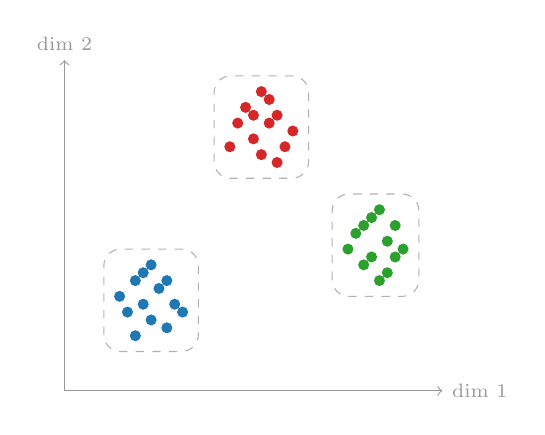
\begin{tikzpicture}[
    dot/.style={circle, inner sep=0pt, minimum size=4pt, thick},
    ann/.style={font=\scriptsize, text=black!55},
]

% Axes
\draw[axiscolor, ->] (0, 0) -- (4.8, 0)
    node[right, font=\scriptsize, text=axiscolor] {dim 1};
\draw[axiscolor, ->] (0, 0) -- (0, 4.2)
    node[above, font=\scriptsize, text=axiscolor] {dim 2};

% Cluster A (blue) -- bottom-left
\foreach \x/\y in {
    1.0/1.1, 1.3/0.8, 0.9/1.4, 1.2/1.3, 1.1/0.9,
    0.8/1.0, 1.4/1.1, 1.0/1.5, 1.3/1.4, 0.7/1.2,
    1.1/1.6, 1.5/1.0, 0.9/0.7} {
    \fill[palA] (\x, \y) circle (2pt);
}

% Cluster B (orange) -- top-center
\foreach \x/\y in {
    2.4/3.2, 2.7/3.5, 2.5/3.0, 2.2/3.4, 2.6/3.7,
    2.8/3.1, 2.3/3.6, 2.9/3.3, 2.5/3.8, 2.1/3.1,
    2.7/2.9, 2.4/3.5, 2.6/3.4} {
    \fill[palB] (\x, \y) circle (2pt);
}

% Cluster C (green) -- right
\foreach \x/\y in {
    3.8/1.6, 4.1/1.9, 3.9/2.2, 4.2/1.7, 3.7/2.0,
    4.0/2.3, 4.3/1.8, 3.8/2.1, 4.1/1.5, 3.6/1.8,
    4.0/1.4, 4.2/2.1, 3.9/1.7} {
    \fill[palC] (\x, \y) circle (2pt);
}

% Annotation
\draw[black!30, dashed, rounded corners=6pt]
    (0.5, 0.5) rectangle (1.7, 1.8);
\draw[black!30, dashed, rounded corners=6pt]
    (1.9, 2.7) rectangle (3.1, 4.0);
\draw[black!30, dashed, rounded corners=6pt]
    (3.4, 1.2) rectangle (4.5, 2.5);

\end{tikzpicture}
\caption{Structured representation.}
\label{fig:viz-guide-good}
\end{subfigure}
\hfill
\begin{subfigure}[t]{0.47\textwidth}
\centering
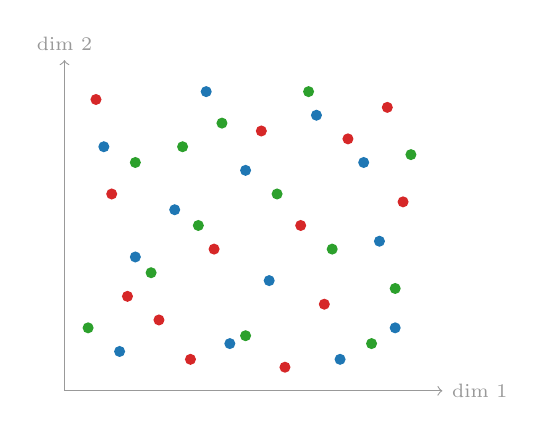
\begin{tikzpicture}[
    dot/.style={circle, inner sep=0pt, minimum size=4pt, thick},
    ann/.style={font=\scriptsize, text=black!55},
]

% Axes
\draw[axiscolor, ->] (0, 0) -- (4.8, 0)
    node[right, font=\scriptsize, text=axiscolor] {dim 1};
\draw[axiscolor, ->] (0, 0) -- (0, 4.2)
    node[above, font=\scriptsize, text=axiscolor] {dim 2};

% Scattered A (blue) -- randomly placed
\foreach \x/\y in {
    0.5/3.1, 2.1/0.6, 3.8/2.9, 1.4/2.3, 4.2/0.8,
    0.9/1.7, 3.2/3.5, 2.6/1.4, 1.8/3.8, 4.0/1.9,
    0.7/0.5, 3.5/0.4, 2.3/2.8} {
    \fill[palA] (\x, \y) circle (2pt);
}

% Scattered B (orange) -- randomly placed
\foreach \x/\y in {
    1.2/0.9, 3.6/3.2, 0.6/2.5, 2.8/0.3, 4.1/3.6,
    1.9/1.8, 0.4/3.7, 3.3/1.1, 2.5/3.3, 1.6/0.4,
    4.3/2.4, 0.8/1.2, 3.0/2.1} {
    \fill[palB] (\x, \y) circle (2pt);
}

% Scattered C (green) -- randomly placed
\foreach \x/\y in {
    2.0/3.4, 3.9/0.6, 1.1/1.5, 4.4/3.0, 0.3/0.8,
    2.7/2.5, 1.5/3.1, 3.4/1.8, 0.9/2.9, 4.2/1.3,
    2.3/0.7, 1.7/2.1, 3.1/3.8} {
    \fill[palC] (\x, \y) circle (2pt);
}

\end{tikzpicture}
\caption{Unstructured representation.}
\label{fig:viz-guide-bad}
\end{subfigure}

\vspace{0.6em}

% Legend
\centering

\begin{tikzpicture}[
    lbl/.style={font=\scriptsize, text=black!55},
]
\fill[palA] (0, 0) circle (2.5pt);
\node[lbl, right] at (0.15, 0) {State property A};
\fill[palB] (2.8, 0) circle (2.5pt);
\node[lbl, right] at (2.95, 0) {State property B};
\fill[palC] (5.6, 0) circle (2.5pt);
\node[lbl, right] at (5.75, 0) {State property C};
\end{tikzpicture}

\caption{Interpreting latent space visualizations. Each point is a
  single state $s_t$ projected to two dimensions via t-SNE or UMAP,
  colored by a game-state property.}
\label{fig:viz-guide}
\end{figure}
